% =====================================================================
% §2 REVISÃO DA LITERATURA
% Arco: como revisamos -> o que existe (taxonomia) -> a lacuna que atacamos
% =====================================================================
\section{Revisão da Literatura}

%%% Frame 2.1 — Revisão sistemática
\begin{frame}{Revisão sistemática}
    \begin{figure}
        \centering
        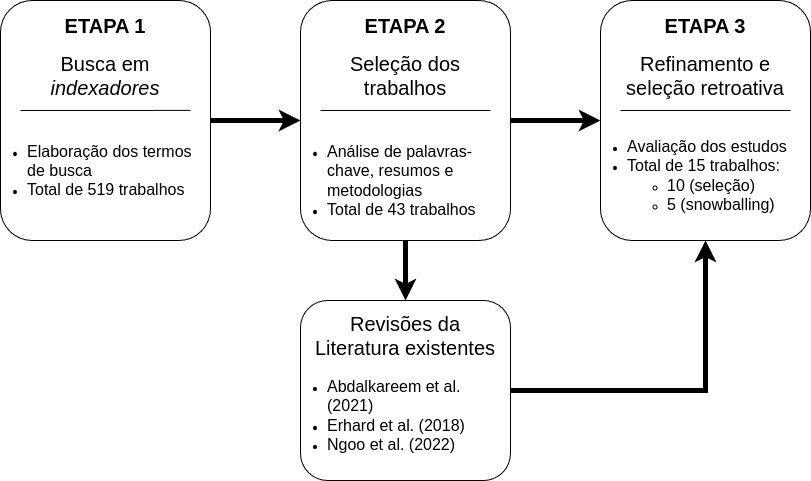
\includegraphics[width=0.92\linewidth]{img/rev-sist-quali.png}
        \caption{Processo da revisão sistemática conduzida no estudo.}
        \label{fig:rev-sistematica}
    \end{figure}
    % TODO: termos-chave, critérios inc./excl., snowballing (Abdalkareem, Erhard, Ngoo).
\end{frame}

%%% Frame 2.2 — Taxonomia dos trabalhos correlatos
\begin{frame}{Trabalhos correlatos: análise taxonômica}
    \begin{figure}
        \centering
        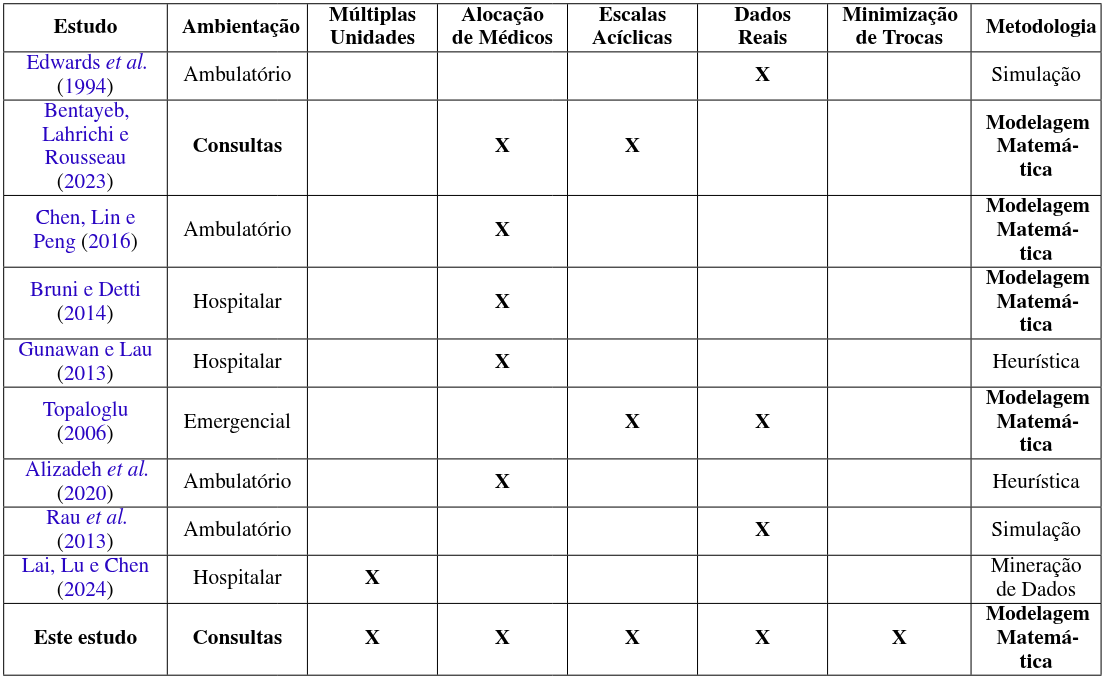
\includegraphics[width=0.9\linewidth]{img/trabalhos-correlatos.png}
        \caption{Análise taxonômica de estudos em PO aplicada ao escalonamento na saúde.}
        \label{fig:taxonomia}
    \end{figure}
    % TODO: destacar colunas onde SÓ este estudo marca X:
    %       múltiplas unidades + minimização de trocas + exames + dados reais.
    % Revisões-base: \cite{Abdalkareem2021_ac,ERHARD20181,Ngoo_Goh_Sze_Sabar_Abdullah_Kendall_2022}
\end{frame}

%%% Frame 2.3 — Lacunas de pesquisa (contexto multiclínica)
\begin{frame}{Lacunas de pesquisa}

    \begin{columns}[T]
        \begin{column}{0.5\textwidth}
            \begin{figure}
                \centering
                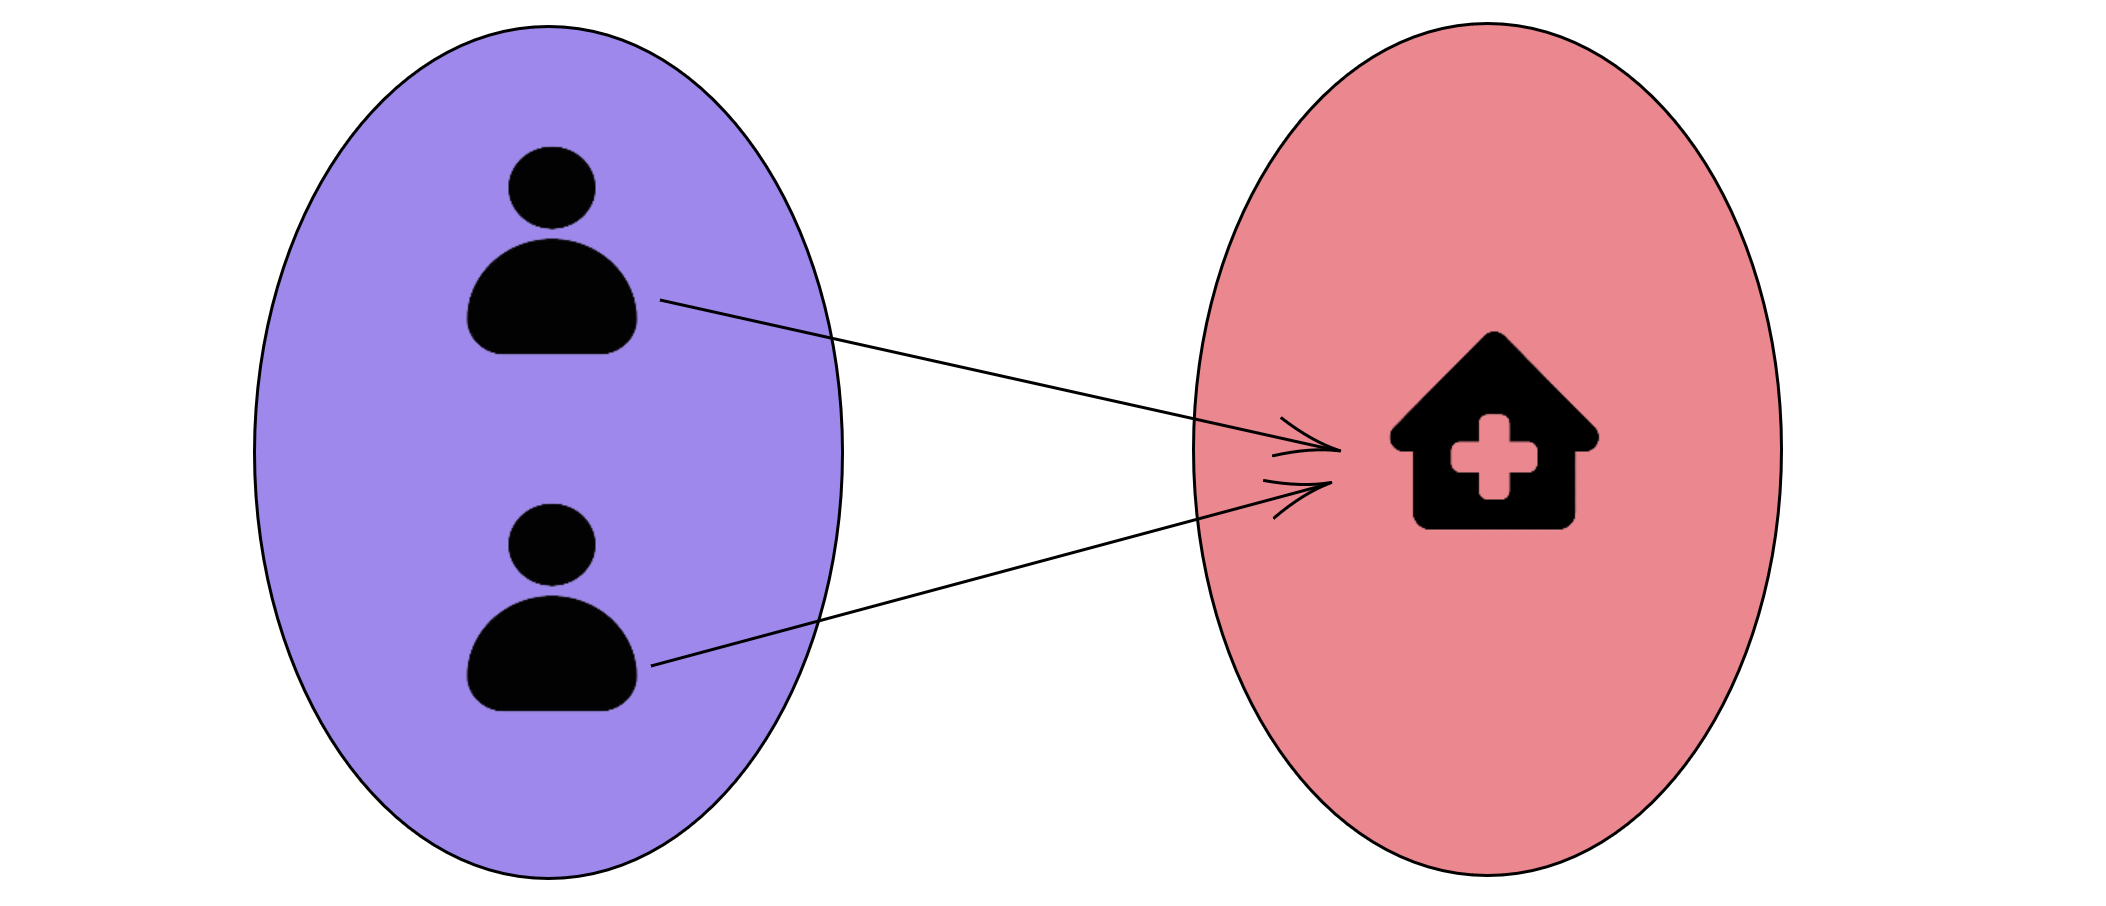
\includegraphics[width=\linewidth]{img/clinic-one-to-m.png}
                \caption{Relação vários-para-um (literatura usual).}
                \label{fig:rel-n-to-1}
            \end{figure}
        \end{column}
        \begin{column}{0.5\textwidth}
            \begin{figure}
                \centering
                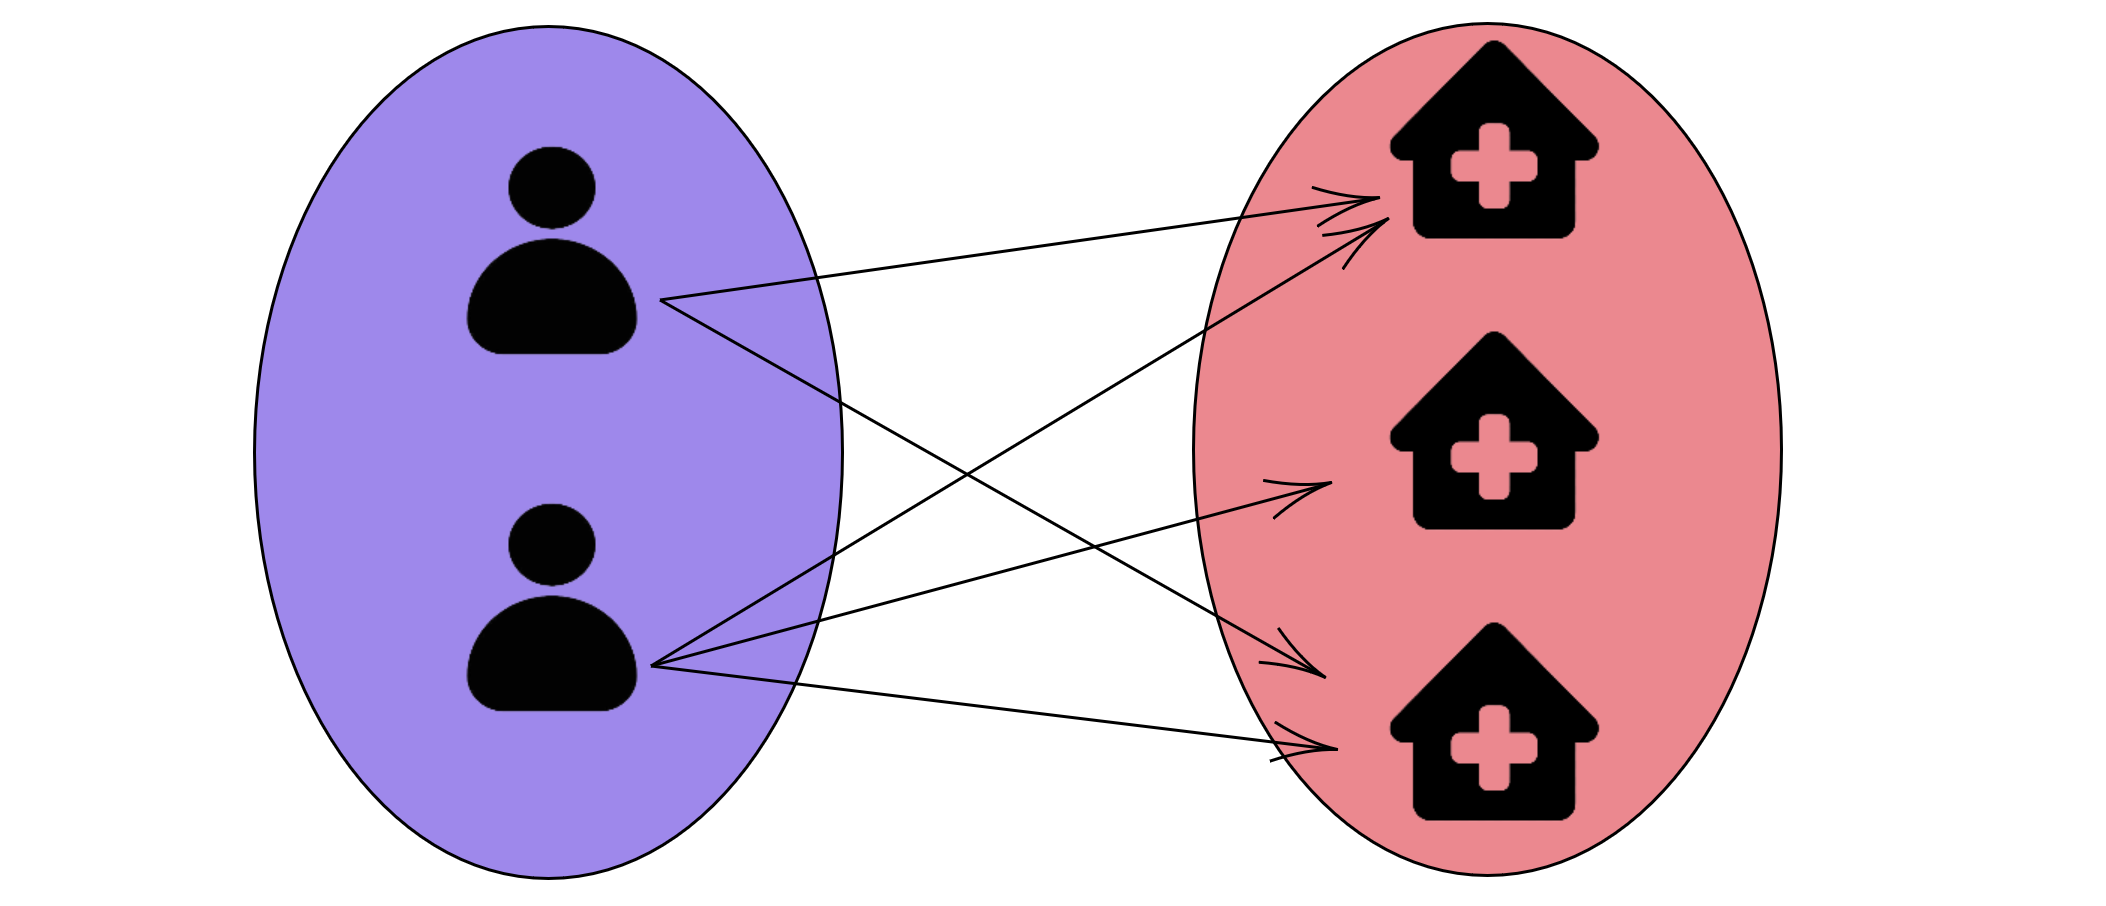
\includegraphics[width=\linewidth]{img/clinic-many-to-many.png}
                \caption{Relação vários-para-vários (este estudo).}
                \label{fig:rel-n-to-n}
            \end{figure}
        \end{column}
    \end{columns}

    \begin{block}{Este trabalho foca portanto...}
        \begin{itemize}
            \item Múltiplas unidades \textbf{autônomas} compartilhando médicos.
            \item Minimização explícita de \textbf{trocas} entre unidades.
            \item Escalas acíclicas, contexto de exames, \textbf{dados reais}.
        \end{itemize}
    \end{block}
\end{frame}
